Il seguente codice MatLab contiene la soluzione del problema dell'Es.9 :\\\
	\lstinputlisting[language=Matlab]{Cap_4/Es_9/Es_9.m}
Le seguenti figura mostrano il polinomio di \textit{Lagrange}, al variare del grado \textit{N} del polinomio con $N=2,4,6,8...40$ :
	\begin{figure}[H]
		\label{Cap_4_Es_9_1}
		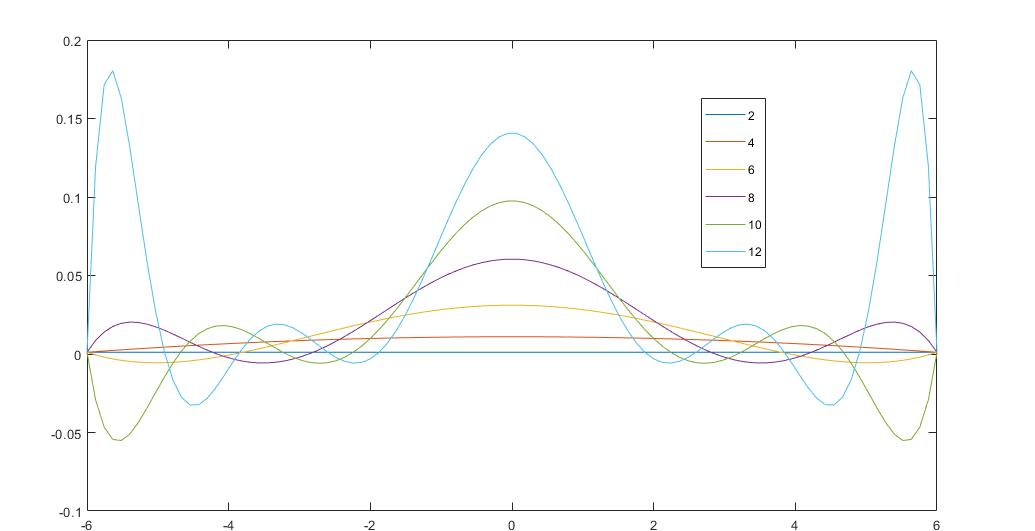
\includegraphics[width=\textwidth]{Plot/Cap_4_Es_9_1}
		\caption*{Polinomio di Lagrange con n° di ascisse $[2,4,6,8,10,12]$}
	\end{figure}
	\begin{figure}[H]
		\label{Cap_4_Es_9_2}
		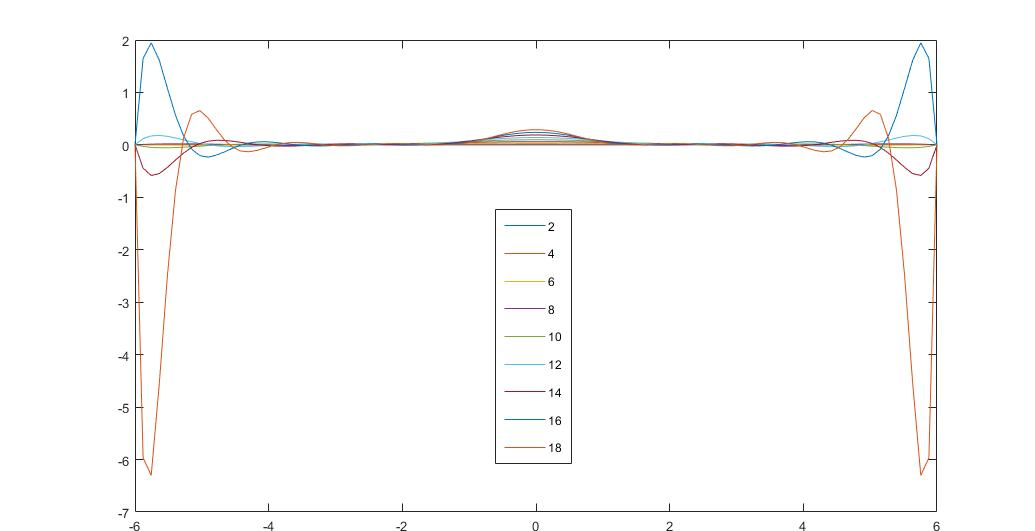
\includegraphics[width=\textwidth]{Plot/Cap_4_Es_9_2}
		\caption*{Polinomio di Lagrange con n° di ascisse $[2,4,6,8,10,12,14,16,18]$}
	\end{figure}
	\begin{figure}[H]
		\label{Cap_4_Es_9_2}
		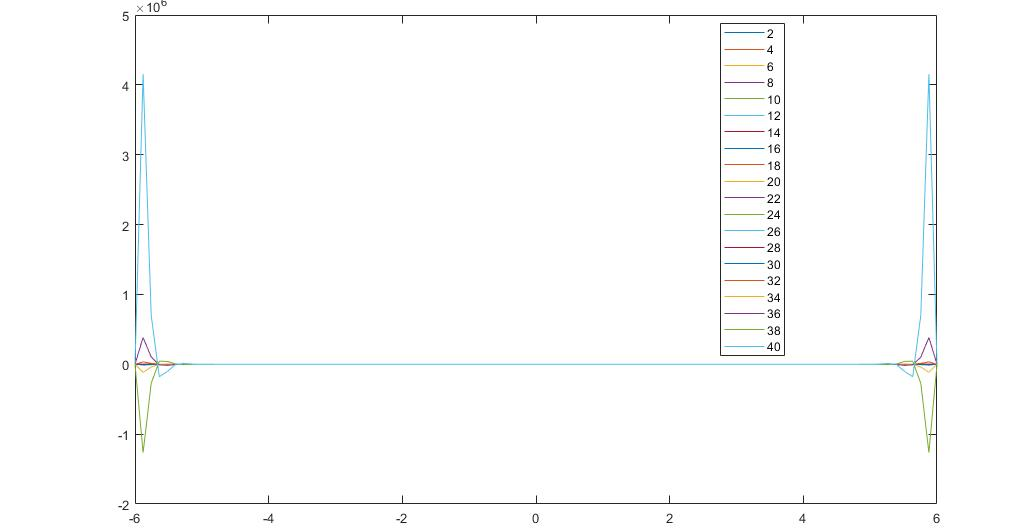
\includegraphics[width=\textwidth]{Plot/Cap_4_Es_9_3}
		\caption*{Polinomio di Lagrange con n° di ascisse $[2,4,6,8,..,40]$}
	\end{figure}
Le seguenti figure mostrano l'andamento della \textit{Spline cubica Naturale} e della \textit{Spline cubica NotAKnot}, al variare del grado \textit{N} del polinomio con $N=2,4,6,8...40$ :\\\


Nella seguente tabella è riportato come varia la \textit{costante di Lebesgue} $\Lambda$, al variare del grado \textit{n} del polinomio e si può notare come la crescita sia \textit{esponenziale}, per $n\rightarrow\infty$, prendendo in cosiderazione \textit{ascisse equidistanti}:\\\
\begin{center}
	\begin{tabular}{|c|c|}
		\hline
		$n$ & $\Lambda$ \\
		\hline
		$2$  & $1.250000000000000$ \\ 
		$4$  & $2.207824277504000$ \\ 
		$6$  & $4.549341110838356$ \\ 
		$8$  & $10.945005461386041$ \\ 
		$10$ & $29.898141093562188$ \\ 
		$12$ & $89.323735973507041$ \\ 
		$14$ & $2.831809493441890e+02$ \\ 
		$16$ & $9.342736404823136e+02$ \\ 
		$18$ & $3.170339307979169e+03$ \\ 
		$20$ & $1.097924392398584e+04$ \\ 
		$22$ & $3.866684343844037e+04$ \\ 
		$24$ & $1.378514896760509e+05$ \\ 
		$26$ & $4.964824917524024e+05$ \\ 
		$28$ & $1.802445465492321e+06$ \\ 
		$30$ & $6.592504744423425e+06$ \\ 
		$32$ & $2.430870357380395e+07$ \\ 
		$34$ & $8.978560703086898e+07$ \\ 
		$36$ & $3.348225693891219e+08$ \\ 
		$38$ & $1.249687039228850e+09$ \\ 
		$40$ & $4.678649708006595e+09$ \\ 
		\hline
	\end{tabular}
\end{center} 
